\documentclass[11pt,a4paper]{article}

\usepackage[margin=0.85in]{geometry}
\usepackage[T1]{fontenc}
\usepackage[utf8]{inputenc}
\usepackage{lmodern}
\usepackage{microtype}
\usepackage{amsmath,amssymb}
\usepackage{booktabs}
\usepackage{graphicx}
\usepackage{array}
\usepackage{enumitem}
\usepackage{xcolor}
\usepackage{parskip}
\usepackage{caption}
\usepackage{hyperref}

\hypersetup{
  colorlinks=true,
  linkcolor=blue!60!black,
  citecolor=blue!60!black,
  urlcolor=blue!60!black,
  pdftitle={Evaluating Decision-Oriented AI for Reliable Software Decisions},
  pdfauthor={Lok Wang Yi (3036067420), Lee Ka Chun (3036841175)}
}

\captionsetup{font=small,labelfont=bf}
\setlength{\tabcolsep}{4pt}
\renewcommand{\arraystretch}{1.15}
\emergencystretch=3em

\title{\textbf{Evaluating Decision-Oriented AI for Reliable Software Decisions}\\[4pt]
\large Empirical Evaluation Across Static Software Operations, Closed-Loop Sequential Control, and In-Context Feedback Adaptation}
\author{Lok Wang Yi (3036067420) $\cdot$ Lee Ka Chun (3036841175) \\ \small COMP7608 Large Language Models --- Group 19}
\date{November 26, 2026}

\begin{document}
\maketitle

\begin{abstract}
\noindent
When AI components select discrete actions inside software systems, strong offline predictive accuracy does not automatically guarantee reliable closed-loop behavior. We evaluate this boundary across three complementary empirical studies with explicit checkpoint provenance and shared reference baselines: (1)~\textbf{Study~1} examines static discrete action selection across an exploratory 4-suite offline benchmark with confidence-gated cloud cascades and a controlled two-student adaptation study on a frozen Software Operations holdout split; (2)~\textbf{Study~2} evaluates closed-loop sequential control in a deterministic, AGX-inspired 4-lap racing simulator (\texttt{RaceEnv}) above a frozen 30\,Hz RL driver, comparing static defaults, domain heuristics, contextual lookup, a compact MLP, and LoRA-adapted Qwen policies alongside a post-hoc 10-model alignment panel; and (3)~\textbf{Study~3} tests in-context adaptation without weight updates across matched no-history ($Z$), actions-only ($A$), and outcome-feedback ($F$) arms. Offline, targeted LoRA adaptation raises local accuracy on the frozen Software Operations holdout to $91.00\%$ ($0.030$ ECE), whereas full fine-tuning of a cross-encoder student fails to improve reliably over its initialization. In closed-loop racing, however, high offline acceptable-set accuracy ($88.56\%$--$92.79\%$) coexists with lower completion than simple non-adaptive controls: none of the evaluated AI models achieved a higher observed completion count than the static control ($41/45$) or domain heuristic ($40/45$) on the matched 45-case panel, and an input-validity audit reveals that right-truncation at $512$ tokens clipped the final option description and \texttt{Answer:} cue on all live-lap Qwen pace calls. Without weight updates, outcome-grounded history yielded three additional completions ($30 \rightarrow 33/45$, $p=0.25$) for the evaluated frontier checkpoint on the 45-case feedback panel, while ungrounded action history degraded an off-the-shelf cross-encoder. Because Study~1A reflects repeated development exposure, Study~2 is bounded to nine fixed track--weather cells (with a live-lap truncation confound in the Qwen pipeline), and the matched panels are small ($N=45$), these findings characterize the tested pipelines and interfaces rather than universal model capabilities.
\end{abstract}

% ============================================================================
\section{Introduction, Model-Identity Matrix, and Three-Study Framing}
% ============================================================================

Integrating a discrete decision-making AI component into a software system introduces a fundamental evaluation question: does high predictive accuracy on recorded decision states translate into reliable behavior once actions alter subsequent states? Across software engineering and autonomous control, an added decision layer can improve outcomes, leave system behavior unchanged, or introduce harmful interventions that degrade reliability relative to a fixed default.

This report organizes the Self-JEV empirical evidence into three complementary studies---linked by \textbf{shared references and explicit checkpoint provenance} rather than one unchanged cohort---under the unifying lens of \textbf{the reliability of a software component that selects discrete actions}:
\begin{itemize}[leftmargin=1.5em,itemsep=2pt]
  \item \textbf{Study~1 (Offline Candidate Selection and Adaptation):} Evaluates discrete action selection across (1A)~a historical/exploratory 4-suite offline benchmark ($N=244$) with confidence-gated cloud cascades and (1B)~a controlled two-student adaptation study on the originally held-out \texttt{holdout\_600} split ($N=600$), plus an additional off-the-shelf MS MARCO MiniLM frozen reference evaluated after the original M2 results were known.
  \item \textbf{Study~2 (Closed-Loop Racing Evaluation, \texttt{racing\_engineer\_v1}):} Uses a reproducible 4-lap racing simulator (\texttt{RaceEnv}) above a frozen 30\,Hz RL driver to evaluate zero-shot transfer, pit-free Stage-B training (\texttt{NN-3}, \texttt{Racing Qwen}, \texttt{lookup\_9cell}), and a complete post-hoc 10-model Stage-B alignment on \texttt{3501..3505} ($N=45$) including raw \texttt{Qwen3.5-0.8B-Base}, \texttt{m2-qwen3.5-0.8b-lora-s42}, \texttt{kev-0.8b}, off-the-shelf MiniLM, and dated \texttt{frontier-llm}.
  \item \textbf{Study~3 (In-Context Feedback and Closed-Loop Reliability, \texttt{F1 v2}):} Evaluates a defined three-model cohort (\texttt{kev-0.8b}, off-the-shelf MiniLM, \texttt{frontier-llm}) on held-out races when supplied with prior-race context under matched no-history ($Z$), actions-only ($A$), and outcome-feedback ($F$) arms ($N=45$, pits enabled).
\end{itemize}

\paragraph{Resolved Model-Identity Provenance.}
Bit-for-bit verification of \nolinkurl{reports/full_benchmark_v2/benchmark_raw.jsonl} against \nolinkurl{reports/full_benchmark/benchmark_raw_self_jev_minilm_packed.jsonl} established that all $244/244$ Study~1A predictions under the UI display label \texttt{self-jev-minilm} ($118/244 = 48.3607\%$) have \textbf{identical probabilities and latencies} to the Run~\#5 trained \textbf{BGE-base ensemble} ($156/313 = 49.84\%$ prior to archiving $69$ historical rank pairs; $156-38=118$). By contrast, the 9-case racing pilot (\texttt{race\_engineer\_v2}), Study~3 (\texttt{F1 v2}), and our alignment supplements loaded off-the-shelf \nolinkurl{cross-encoder/ms-marco-MiniLM-L6-v2} ($22.7$M, not fine-tuned for this project)~\cite{minilm_card}. Table~\ref{tab:master_model_matrix} assigns a separate row to each distinct checkpoint or model identity across all studies.

\begin{table}[t]
\centering
\caption{Master Model-Identity and Cross-Study Role Matrix. Each row maps an exact checkpoint/interface to the studies where it was evaluated, separating Run~\#5 BGE-base ensemble, off-the-shelf MS MARCO MiniLM, BGE zero-shot initialization vs.\ trained BGE student, and build-only \texttt{car-build-nn}/\texttt{nn-combo} vs.\ two-head \texttt{NN-3}.}
\label{tab:master_model_matrix}
\resizebox{\textwidth}{!}{%
\begin{tabular}{llccccc}
\toprule
Experimental Identity & Exact Checkpoint / Interface & Study 1A & Study 1B & Study 2 Bridge & Study 2 Stage B & Study 3 \\
 & & ($N=244$) & ($N=600$) & ($N=9/27$, Pits ON) & ($N=180/45$, Pits OFF) & ($N=45$, Pits ON) \\
\midrule
\texttt{frontier-llm} (dated cloud ref.) & \texttt{deepseek-v4.1-flash-1017} (API JSON) & Yes & Yes (orig ref) & --- & Yes (Align-45) & Yes ($Z/A/F$) \\
\texttt{kev-0.8b} (frozen local) & \texttt{jaredpalmer/kev-0.8b} (pointer scorer) & Yes & Yes & Yes ($N=9$) & Yes (Align-45) & Yes ($Z/A/F$) \\
Run~\#5 BGE ensemble & Trained BGE-base ensemble (v1 packed) & Yes (48.36\%) & --- & --- & --- & --- \\
Off-the-shelf MiniLM & \texttt{cross-encoder/ms-marco-MiniLM-L6-v2} & --- & Yes (post-hoc ref) & Yes ($N=9$) & Yes (Align-45) & Yes ($Z/A/F$) \\
\texttt{Raw Qwen Base} & \texttt{Qwen/Qwen3.5-0.8B-Base} (letter logits) & Yes (\texttt{-ll}) & Yes (zero-shot) & Yes ($N=9$) & Yes (Align-45) & --- \\
\texttt{M2 Ops Qwen LoRA} & \texttt{m2-qwen3.5-0.8b-lora-s42} ($r=16$, $T=2.02$) & --- & Yes (91.00\%) & Yes ($N=9, 27$) & Yes (Align-45) & --- \\
\texttt{Racing Qwen LoRA} & \texttt{qwen\_lora\_racing\_v1} (s2026, $T=1.47$) & --- & --- & --- & Yes ($N=45$ Fresh/Hist) & --- \\
\texttt{M2 BGE Zero-Shot} & \texttt{BAAI/bge-reranker-base} (init., $T=6.15$) & --- & Yes (19.67\%) & --- & --- & --- \\
\texttt{M2 BGE Trained} & \texttt{bge\_trained\_deploy} (s1024 + 3-seed FT) & --- & Yes (22.17\% / 20.72\%) & --- & --- & --- \\
\texttt{car-build-nn} / \texttt{nn-combo} & Build-only numeric MLP (12-feat.\ + driver) & Yes (S3 only) & --- & Yes ($N=9$) & --- & Ref (\texttt{nn-combo}) \\
\texttt{NN-3} (\texttt{nn3\_racing\_v1}) & Separate build (11-feat.) / pace (29-feat.) 2-hidden-layer MLPs & --- & --- & --- & Yes ($N=180/45$) & --- \\
Sim controls \& lookup & \texttt{driver\_only}, \texttt{track\_rule}, \texttt{lookup\_9cell} & --- & --- & Yes & Yes ($N=180/45$) & Refs \\
\bottomrule
\end{tabular}}
\end{table}

% ============================================================================
\section{Study 1: Offline Candidate Selection and Adaptation}
% ============================================================================

Study~1 establishes the offline decision-quality baseline in two stages with distinct evidential roles: (1)~\textbf{Study~1A} is a \textbf{historical/exploratory evaluation of the retained benchmark items} (\texttt{full\_benchmark\_v2}, $N=244$, filtered from an earlier 313-item benchmark that was inspected across repeated development runs), comparing eight local, cross-encoder, specialist, and frontier models plus confidence-gated cloud cascades; and (2)~\textbf{Study~1B} is a controlled two-student adaptation experiment (\texttt{M2 V5}) on the originally held-out \texttt{holdout\_600} Software Operations split ($N=600$), supplemented by an additional off-the-shelf MS MARCO MiniLM frozen reference evaluated after the original M2 results were known. Across both stages, systems are scored on accuracy, option-order swap sensitivity (order-flip rate), output validity, 10-bin expected calibration error (ECE)~\cite{guo2017calibration}, area under the risk--coverage curve (AURC)~\cite{geifman2017selective}, and inference latency.

\subsection{Study 1A: Exploratory Multi-Suite Offline Benchmark v2 (\texorpdfstring{$N=244$}{N=244}) and Cloud Cascades}

The retained \texttt{full\_benchmark\_v2} benchmark ($N=244$) spans four domains: \textbf{Suite~1 (Software Ops, $n=120$)}, \textbf{Suite~2 (Engineering Evidence Discipline, $n=18$)} (69 historical rank pairs archived from the earlier 313-item benchmark), \textbf{Suite~3 (Car Build, $n=34$; clean subset $n=28$)}, and \textbf{Suite~4 (Stress Test, $n=72$)}. Because removing the 69 historical rank pairs does not restore an untouched test set after repeated development inspection of the v1 benchmark, Study~1A serves as an exploratory benchmark rather than an untouched confirmatory holdout. Prompts also stratify across three context-length bands: Short ($<400$ tokens, $n=178$), Medium ($400$--$1000$, $n=30$), and Long ($>1000$, $n=36$). Table~\ref{tab:study1a_bench} summarizes overall performance, per-suite accuracy, calibration, order-flip stability, and latency across all eight evaluated systems.

\begin{table}[t]
\centering
\caption{Study~1A (Exploratory): Multi-suite offline benchmark v2 ($N=244$ retained items, 95\% bootstrap CIs). \texttt{car-build-nn} is a domain specialist evaluated strictly on Suite~3 ($n=34$, clean $n=28$: $82.1\%$). Provenance audit confirmed that the \texttt{self-jev-minilm} row ($118/244 = 48.36\%$) is the Run~\#5 trained BGE-base ensemble filtered from v1 ($156/313$), \emph{not} off-the-shelf MS MARCO MiniLM.}
\label{tab:study1a_bench}
\resizebox{\textwidth}{!}{%
\begin{tabular}{lcccccccccc}
\toprule
System & Overall Acc [95\% CI] & S1 & S2 & S3 & S4 & ECE & AURC & Flip & Valid & p50 (ms) \\
 & & ($n=120$) & ($n=18$) & ($n=34$) & ($n=72$) & & & & & \\
\midrule
\texttt{frontier-llm} & \textbf{95.08\%} [92.2, 97.5] & 100.0\% & 100.0\% & 64.7\% & 100.0\% & 0.043 & 0.006 & 2.05\% & 100.0\% & 561.1 \\
\texttt{kev-0.8b} & 62.30\% [56.2, 68.4] & 68.3\% & 94.4\% & 41.2\% & 54.2\% & 0.235 & 0.165 & 33.20\% & 100.0\% & 49.9 \\
Run~\#5 BGE ens.\ (\texttt{self-jev-minilm}) & 48.36\% [42.2, 54.9] & 67.5\% & 16.7\% & 26.5\% & 34.7\% & 0.077 & 0.310 & 0.00\% & 100.0\% & 75.2 \\
\texttt{self-jev-v2-m3} & 40.57\% [34.4, 47.1] & 53.3\% & 50.0\% & 20.6\% & 26.4\% & 0.080 & 0.322 & 0.00\% & 100.0\% & 250.7 \\
\texttt{self-jev-v2.1-m3} & 38.11\% [32.4, 43.9] & 54.2\% & 33.3\% & 20.6\% & 20.8\% & 0.058 & 0.385 & 0.00\% & 100.0\% & 208.4 \\
\texttt{qwen-0.8b-ll} & 26.64\% [20.9, 32.4] & 26.7\% & 27.8\% & 29.4\% & 25.0\% & 0.226 & 0.616 & 21.31\% & 99.59\% & 1914.4 \\
\texttt{qwen-0.8b-json} & 23.36\% [18.0, 28.7] & 33.3\% & 0.0\% & 35.3\% & 6.9\% & 0.473 & 0.718 & 65.16\% & 75.00\% & 854.5 \\
\midrule
\texttt{car-build-nn} (S3 only) & 79.41\% [64.7, 91.2] & --- & --- & \textbf{79.4\%} & --- & 0.115 & 0.097 & --- & 100.0\% & 0.032 \\
\bottomrule
\end{tabular}}
\end{table}

Four findings emerge from Study~1A:
\begin{enumerate}[leftmargin=1.5em,itemsep=2pt]
  \item \textbf{Large frontier--local gap across the evaluated local systems:} \texttt{frontier-llm} ($95.08\%$, \$0.4049/1k calls) significantly outperforms \texttt{kev-0.8b} ($62.30\%$; exact two-sided binomial McNemar $90$ vs.\ $10$, $p < 10^{-6}$), while \texttt{kev-0.8b} significantly outperforms the Run~\#5 BGE ensemble (\texttt{self-jev-minilm}, $48.36\%$; $48$ vs.\ $14$ discordant items, exact two-sided binomial McNemar $p = 1.74\times 10^{-5}$; continuity-corrected $\chi^2$ approximation $p = 2.78\times 10^{-5}$) and \texttt{qwen-0.8b-ll} ($26.64\%$; $95$ vs.\ $8$, exact $p < 10^{-6}$). Across context lengths, \texttt{self-jev-minilm} degrades sharply from Short ($56.2\%$) to Medium ($30.0\%$) and Long ($25.0\%$), whereas \texttt{frontier-llm} reaches $100.0\%$ on both Medium and Long prompts.
  \item \textbf{Scoring interface and order-flip fragility:} When each candidate is scored independently with unchanged paired inputs, the score vector can be permutation-equivariant, though the selected argmax can still flip through candidate-dependent formatting, tied or near-tied scores, numerical effects, or index-based tie-breaking (as later observed in Study~1B's BGE runs). On these specified Study~1A runs, the three cross-encoders (\texttt{self-jev-minilm}, \texttt{v2-m3}, \texttt{v2.1-m3}) exhibited $0.00\%$ observed flips. By contrast, free-form JSON generation (\texttt{qwen-0.8b-json}) fails schema parsing on $25.0\%$ of items ($75.00\%$ valid) and flips on $65.16\%$ of swapped prompts, whereas direct option log-likelihood scoring (\texttt{qwen-0.8b-ll}) restores $99.59\%$ validity and cuts flips to $21.31\%$.
  \item \textbf{Compact domain specialists excel on numeric structure:} On Suite~3 (Car Build, $n=34$), the tiny \texttt{car-build-nn} MLP ($79.41\%$, clean $82.1\%$, $0.032$\,ms p50) significantly outperforms \texttt{kev-0.8b} ($15$ vs.\ $2$, exact $p = 0.00235$), \texttt{qwen-0.8b-ll} ($19$ vs.\ $2$, exact $p = 0.00022$), and \texttt{self-jev-minilm} ($20$ vs.\ $2$, exact $p = 0.00012$). Against \texttt{frontier-llm} ($64.7\%$; clean $78.6\%$), \texttt{car-build-nn} achieved a higher observed Suite~3 score at $>17{,}000\times$ lower latency, though the paired difference ($10$ vs.\ $5$ discordant items, exact $p = 0.3018$) is not statistically significant and does not establish equivalence.
  \item \textbf{Confidence-gated cloud cascades require both ranking quality and non-degenerate confidence support:} As shown in Table~\ref{tab:study1a_cascade}, escalating the lowest-confidence items from \texttt{kev-0.8b} (AURC $0.165$) to \texttt{frontier-llm} recovers $89.3\%$ accuracy at $50.0\%$ actual escalation and $94.7\%$ at $79.9\%$ actual escalation. At $50.0\%$ actual escalation, \texttt{qwen-0.8b-ll -> frontier-llm} reaches only $68.0\%$. By contrast, \texttt{qwen-0.8b-json -> frontier-llm} exhibits a sharp mismatch between \emph{target} and \emph{achieved} escalation: $61/244$ parse failures (\texttt{conf}$=0.0$) impose a $25.0\%$ mandatory escalation floor ($48.36\%$ accuracy, $118/244$), and because valid outputs pile up on a tied verbalized confidence of $0.95$, strict thresholding ($\text{conf} < \tau$) fixes $\tau = 0.9500$ across all targets from $40\%$ through $90\%$. Consequently, \textbf{actual escalation caps at $35.66\%$ ($87/244$)} and accuracy plateaus at $51.64\%$ ($126/244$) across target rates $40\%$--$90\%$, jumping to $95.08\%$ ($232/244$) only when $\tau=2.0$ forces $100.0\%$ actual escalation.
\end{enumerate}

\begin{table}[t]
\centering
\caption{Study~1A: Confidence-gated cloud cascades on \texttt{full\_benchmark\_v2} ($N=244$), distinguishing target escalation from actual achieved escalation under strict $\text{conf} < \tau$ routing. For \texttt{qwen-0.8b-json}, tied verbalized confidence ($0.95$) caps actual escalation at $35.66\%$ ($87/244$) for targets $40\%$--$90\%$.}
\label{tab:study1a_cascade}
\resizebox{\textwidth}{!}{%
\begin{tabular}{ccccccc}
\toprule
Target & \multicolumn{3}{c}{\texttt{kev-0.8b -> frontier-llm}} & \multicolumn{3}{c}{\texttt{qwen-0.8b-json -> frontier-llm}} \\
\cmidrule(lr){2-4}\cmidrule(lr){5-7}
Escalation & Actual Esc. & Acc & Cost (\$/1k) & Actual Esc. & Acc & Cost (\$/1k) \\
\midrule
0\% (local) & 0.0\% (0/244) & 62.3\% & \$0.0000 & 25.0\% (61/244) & 48.4\% & \$0.2463 \\
20\% & 19.7\% (48/244) & 73.8\% & \$0.0676 & 25.0\% (61/244) & 48.4\% & \$0.2463 \\
30\% & 29.9\% (73/244) & 79.5\% & \$0.1246 & 29.9\% (73/244) & 51.6\% & \$0.2534 \\
50\% & 50.0\% (122/244) & 89.3\% & \$0.2695 & 35.7\% (87/244) & 51.6\% & \$0.2602 \\
60\% & 59.8\% (146/244) & 91.4\% & \$0.2827 & 35.7\% (87/244) & 51.6\% & \$0.2602 \\
80\% & 79.9\% (195/244) & 94.7\% & \$0.3609 & 35.7\% (87/244) & 51.6\% & \$0.2602 \\
90\% & 89.8\% (219/244) & 95.1\% & \$0.3908 & 35.7\% (87/244) & 51.6\% & \$0.2602 \\
100\% (cloud) & 100.0\% (244/244) & 95.1\% & \$0.4049 & 100.0\% (244/244) & 95.1\% & \$0.4049 \\
\bottomrule
\end{tabular}}
\end{table}

\subsection{Study 1B: Controlled Two-Student Adaptation (\texttt{M2 V5}, \texttt{holdout\_600})}

To test whether targeted task adaptation closes the frontier--local gap on static Software Operations decisions without losing calibration, Study~1B trained two student architectures under identical data and split isolation: (1)~\texttt{BAAI/bge-reranker-base} ($278.0$M parameters, full fine-tuning with FP16 AMP autocast, $5.62$\,GB peak allocated GPU memory, $\approx 948$\,s/seed) and (2)~\texttt{Qwen/Qwen3.5-0.8B-Base} ($752.4$M frozen backbone loaded in FP16 on Colab T4, $\approx 1.50$\,GB weights, with $6.39$M trainable rank-16 LoRA adapters stored in FP32 and FP16 mixed-precision forward/backward autocast; $1.81$\,GB peak allocated PyTorch GPU tensor memory via \texttt{torch.cuda.max\_memory\_allocated()}, excluding CUDA driver/caching-allocator overhead; $\approx 3118$\,s/seed; local CPU inference loads the base in FP32). Both students were trained across three random seeds ($42, 1024, 2026$) on Colab Tesla T4 using gold-verified hard labels from \texttt{deepseek-v4.1-flash-1017} ($833/840$ training items retained after excluding $7$ teacher--gold disagreements; SHA-256 \texttt{2146a5b460e1da11}).

\paragraph{Training Objectives and Optimization.}
In \texttt{scripts/train\_m2\_v5\_students.py}, both students were trained for four epochs with seeds $42, 1024$, and $2026$ using AdamW ($\text{weight\_decay}=0.01$), $10\%$ linear warmup followed by cosine learning-rate decay, and gradient accumulation over eight one-decision microbatches.

For \texttt{M2 Ops Qwen LoRA}, the FP16 base weights were frozen and FP32 LoRA adapters~\cite{hu2022lora} were trained with rank $r=16$, scaling parameter $\alpha=32$, dropout $0.05$, and learning rate $2\times 10^{-4}$. Adapters targeted linear modules matching \texttt{q\_proj}, \texttt{k\_proj}, \texttt{v\_proj}, \texttt{o\_proj}, \texttt{gate\_proj}, \texttt{up\_proj}, and \texttt{down\_proj}. The objective was cross-entropy over the $K$ candidate-letter logits at the final retained prompt position, with random option-order permutation resampled on every presentation of a training example (remapping the gold target to its corresponding letter index).

For \texttt{M2 BGE Student}, all $278.0$M parameters were fine-tuned at learning rate $2\times 10^{-5}$ under FP16 AMP autocast. Each context--question and candidate pair was encoded independently to obtain one scalar score, and cross-entropy was applied across the complete $K$-candidate score list for each decision.

\paragraph{Calibration and Selection Sequence.}
In \texttt{scripts/train\_m2\_v5\_students.py}, model selection followed a fixed three-step sequence: (i)~for each seed, the best epoch was chosen by lowest \emph{uncalibrated} NLL on \texttt{dev\_180} (\texttt{832a24c856ed194b}) and saved; (ii)~a scalar temperature $T$ was fitted on \texttt{cal\_180} (\texttt{8c8f19e4dcbcb59a}) for each seed's saved checkpoint; and (iii)~each seed's temperature-calibrated checkpoint was re-evaluated on \texttt{dev\_180}, and the single deployment seed was selected by lowest \emph{calibrated} \texttt{dev\_180} NLL (meaning the fitted temperatures can influence which seed wins) before freezing weights and $T$ for a single evaluation on the originally held-out \texttt{holdout\_600} split ($N=600$, SHA-256 \texttt{3782d9f6ba4a4164}). The off-the-shelf MS MARCO MiniLM row in Tables~\ref{tab:study1_holdout}--\ref{tab:study1b_breakdown} is an \textbf{additional frozen reference evaluated after the original M2 results were known} ($T=6.15$ fitted on \texttt{cal\_180}); it provides a cross-study anchor rather than inheriting the original experiment's untouched-confirmation status without qualification.

\begin{table}[t]
\centering
\caption{Study~1B: Controlled two-student evaluation on frozen \texttt{holdout\_600} ($N=600$), plus an additional off-the-shelf MS MARCO MiniLM frozen reference evaluated post-hoc ($T=6.15$ fitted on \texttt{cal\_180}). Frontier teacher (\texttt{deepseek-v4.1-flash-1017}) is an independent-gold reference (orig-only; API returns text confidence rather than option probabilities, so NLL/ECE/AURC are omitted).}
\label{tab:study1_holdout}
\resizebox{\textwidth}{!}{%
\begin{tabular}{lcccccccc}
\toprule
System & Acc (Orig) & Acc (Swap) & Flip Rate & NLL & ECE & AURC & Err AUROC & p50 (ms) \\
\midrule
Off-the-shelf MiniLM (post-hoc ref., $T=6.15$) & 17.83\% & 17.83\% & 0.00\% & 1.659 & 0.103 & 0.825 & 0.483 & 32.1 \\
\texttt{bge\_zeroshot} ($T=6.15$) & 19.67\% & 19.67\% & 0.17\% & 1.634 & 0.077 & 0.802 & 0.506 & 24.6 \\
\texttt{bge\_trained\_deploy} (s1024, $T=0.65$) & 22.17\% & 23.17\% & 5.83\% & 1.625 & 0.040 & 0.770 & 0.562 & 24.9 \\
\quad\emph{BGE 3-seed descriptive mean $\pm$ sd} & 20.72\% $\pm$ 1.02 & 20.89\% $\pm$ 1.61 & 63.33\% $\pm$ 41.17 & 1.626 $\pm$ 0.008 & 0.056 $\pm$ 0.017 & 0.795 $\pm$ 0.019 & --- & --- \\
\texttt{qwen\_zeroshot} ($T=6.15$) & 28.33\% & 28.33\% & 88.17\% & 1.583 & 0.052 & 0.652 & 0.630 & 145.3 \\
\texttt{kev-0.8b} (frozen, $T=1.00$) & 62.50\% & 58.50\% & 19.33\% & 1.133 & 0.177 & 0.287 & 0.715 & 258.3 \\
\texttt{m2-qwen3.5-0.8b-lora} (s42, $T=2.02$) & \textbf{91.00\%} & \textbf{88.50\%} & \textbf{7.33\%} & \textbf{0.271} & \textbf{0.030} & \textbf{0.026} & \textbf{0.881} & 168.0 \\
\quad\emph{Qwen LoRA 3-seed descriptive mean $\pm$ sd} & 89.50\% $\pm$ 1.22 & 86.56\% $\pm$ 1.80 & 8.78\% $\pm$ 1.49 & --- & 0.047 $\pm$ 0.013 & 0.032 $\pm$ 0.006 & --- & --- \\
\midrule
Frontier Teacher (ref., orig-only) & 100.00\% & --- & --- & --- & --- & --- & --- & 793.6 \\
\bottomrule
\end{tabular}}
\end{table}

\begin{table}[t]
\centering
\caption{Study~1B: Per-bucket ($n=150$ each), prompt-wrapper (Clean $n=448$ / Wrapped $n=152$), and abstention audit ($128$ gold abstain / $472$ non-abstain) on \texttt{holdout\_600}. FAR denotes False Abstention Rate.}
\label{tab:study1b_breakdown}
\resizebox{\textwidth}{!}{%
\begin{tabular}{lccccccccc}
\toprule
System & \texttt{api\_rout.} & \texttt{eng\_trade.} & \texttt{inc\_triage} & \texttt{rel\_gate} & Clean & Wrapped & Abst.\ Rec & Abst.\ Prec & FAR \\
\midrule
Off-the-shelf MiniLM (post-hoc) & 18.7\% & 14.0\% & 21.3\% & 17.3\% & 18.1\% & 17.1\% & 18.0\% & 15.0\% & 27.5\% \\
\texttt{qwen\_zeroshot} & 46.7\% & 22.7\% & 24.0\% & 20.0\% & 27.5\% & 30.9\% & 15.6\% & 33.3\% & 8.5\% \\
\texttt{kev-0.8b} (frozen) & 90.7\% & 84.7\% & 51.3\% & 23.3\% & 62.9\% & 61.2\% & 41.4\% & 65.4\% & 5.9\% \\
\texttt{m2-qwen-lora-s42} & \textbf{97.3\%} & 78.0\% & \textbf{89.3\%} & \textbf{99.3\%} & \textbf{92.0\%} & \textbf{88.2\%} & \textbf{89.8\%} & \textbf{87.8\%} & \textbf{3.4\%} \\
Frontier Teacher (ref.) & 100.0\% & 100.0\% & 100.0\% & 100.0\% & 100.0\% & 100.0\% & 100.0\% & 100.0\% & 0.0\% \\
\bottomrule
\end{tabular}}
\end{table}

Tables~\ref{tab:study1_holdout} and~\ref{tab:study1b_breakdown} highlight three main conclusions from Study~1B:
\begin{enumerate}[leftmargin=1.5em,itemsep=2pt]
  \item \textbf{Strong local adaptation and calibration with LoRA:} Selected \texttt{m2-qwen3.5-0.8b-lora-s42} reaches $91.00\%$ ($546/600$) original accuracy, $88.50\%$ swapped accuracy, $7.33\%$ flip rate, $0.030$ ECE, $0.026$ AURC, and $0.881$ error-detection AUROC at $168.0$\,ms p50 ($4.7\times$ faster than the $793.6$\,ms frontier teacher; $1075.6$\,ms teacher p95). Across seeds ($42/1024/2026$: $91.0\% / 88.0\% / 89.5\%$), Qwen LoRA is stable ($89.50\% \pm 1.22\%$), significantly beating \texttt{qwen\_zeroshot} ($385$ vs.\ $9$, exact $p < 10^{-6}$) and \texttt{kev-0.8b} ($206$ vs.\ $35$, exact $p < 10^{-6}$), while still trailing the $100.0\%$ ($600/600$) frontier teacher ($54$ vs.\ $0$, exact $p < 10^{-6}$).
  \item \textbf{Architecture- and optimization-dependent failure mode (BGE collapse):} The tested full fine-tuning configuration of \texttt{BAAI/bge-reranker-base} failed to learn the 5-way decision boundary, exhibiting severe seed-dependent order-flip collapse: seed~42 ($20.0\%$ acc, $100.0\%$ flip), seed~1024 ($22.17\%$ acc, $5.83\%$ flip), and seed~2026 ($20.0\%$ acc, $84.17\%$ flip). We report the descriptive and paired statistics separately: the three-seed descriptive mean is $20.72\% \pm 1.02\%$, while comparing the selected seed~1024 deployment checkpoint ($133/600 = 22.17\%$) against \texttt{bge\_zeroshot} ($118/600 = 19.67\%$) yields $105$ vs.\ $90$ discordant pairs (exact two-sided McNemar $p = 0.3161$), which does not establish a statistically significant difference (nor equivalence).
  \item \textbf{Operational robustness across buckets, wrappers, and abstention:} \texttt{m2-qwen-lora-s42} gains most sharply on structured operational gates where frozen \texttt{kev-0.8b} struggles (\texttt{release\_gate}: $23.3\% \rightarrow 99.3\%$; \texttt{incident\_triage}: $51.3\% \rightarrow 89.3\%$), retains high accuracy under prompt wrappers ($92.0\%$ Clean vs.\ $88.2\%$ Wrapped), and raises abstention recall from $41.4\%$ to $89.8\%$ ($87.8\%$ precision) while lowering False Abstention Rate to $3.4\%$ ($91.3\%$ non-abstain accuracy).
\end{enumerate}

\paragraph{Model Selection and Cross-Study Reference Roles.}
Study~1 provides empirical context for the text and numeric approaches examined in Study~2. The \texttt{M2 Ops Qwen LoRA} checkpoint achieved $91.00\%$ accuracy and $0.030$ ECE, supporting further investigation of the Qwen base-model and LoRA approach; \texttt{Racing Qwen} initialized a fresh adapter on the base checkpoint and trained it on racing data. The tested BGE full fine-tuning configuration was not extended to racing after failing to establish an improvement over initialization. Separately, the strong Suite~3 result of the build-only \texttt{car-build-nn} ($79.41\%$ at $0.032$\,ms) motivated including a newly trained numeric racing policy, \texttt{NN-3}.

Existing checkpoints provided frozen references in the transfer pilots and subsequent Stage-B alignment supplement, with participation recorded in Table~\ref{tab:master_model_matrix}. \texttt{M2 Ops Qwen LoRA} tested cross-domain transfer from Software Operations; \texttt{Raw Qwen Base} provided the unadapted initialization reference; \texttt{kev-0.8b} and off-the-shelf MiniLM provided local decision-scoring and cross-encoder references; and \texttt{frontier-llm} was added as a dated cloud reference in the post-hoc alignment supplement.

% ============================================================================
\section{Study 2: Closed-Loop Racing Evaluation (\texttt{RaceEnv})}
% ============================================================================

Study~1 evaluated decision quality on fixed inputs. Study~2 extends the evaluation to closed-loop racing, where actions affect subsequent states, through two complementary comparisons: direct transfer of frozen checkpoints and evaluation of separately trained text and numeric racing policies.

\subsection{Construction and Calibration of the AGX-Inspired Simulator}

Observational analysis of $56$ historical AGX match logs (\texttt{pace\_accuracy\_summary.json}) showed $37/56$ classified attempts and $28/51$ reference-applicable full 4-lap finishes (median gap $175.9$\,s / $41.78\%$ behind external AGX winners), where uncontrolled opponent, weather, and hardware variation prevents causal attribution of high-level decisions. To enable reproducible, paired closed-loop evaluation and exact counterfactual rollout labeling, we built a clean-room, AGX-inspired racing simulator (\texttt{self\_jev/sim}) alongside a separate standalone 4-wheel reference verification engine (\texttt{mac\_racing\_sim}):
\begin{itemize}[leftmargin=1.5em,itemsep=2pt]
  \item \textbf{Track Geometry and Sporting Rules (\texttt{env.py}):} Track centerlines are loaded directly from official \texttt{agx-racing-kit} mapdata for \texttt{parkland} ($5795.8$\,m), \texttt{highland} ($6999.4$\,m), and \texttt{crossover} ($5803.2$\,m) at uniform $\approx 2.0$\,m arc-length spacing, encoding curvature, grade, banking, track half-widths, aero zones, pit entry/exit coordinates, and Frenet $(s, n)$ projection. \texttt{RaceEnv} enforces dynamic wetness ramps, $35.766$\,s pit-lane transit/service (resetting tyre wear to $0.00$), wall graze versus fatal wall retirement ($v_{\text{lat}} \ge 12.0$\,m/s), 30\,s ring-buffer stall detection, and race time limits, while supporting exact single-world state snapshot/restore for counterfactual rollouts.
  \item \textbf{Batched Vehicle Physics (\texttt{physics.py}):} A PyTorch-vectorized dynamic bicycle model runs at $30$\,Hz ($\Delta t = 1/30$\,s) with $4$ internal physics substeps per step ($120$\,Hz integration). It models a $550$\,kW ICE and $350$\,kW ERS hybrid powertrain ($120$\,kW harvest, $120$\,kW override, $4.0$\,MJ SoC window, speed-dependent deployment taper), $54$\,kN max braking, wing-scaled aero drag/downforce with $22\%$ active-aero drag cut, nonlinear $\tanh$ lateral tyre saturation with traction-circle longitudinal capping, and compound-specific grip (\texttt{soft} $1.72$, \texttt{medium} $1.64$, \texttt{hard} $1.56$) modulated by wetness (\texttt{wet\_grip\_drop} $= 0.30$), wear, and thermal dynamics (\texttt{self\_jev/sim/calibrated\_params.json}).
  \item \textbf{Calibration Scope and Companion Reference Engine:} \texttt{RaceEnv}'s bicycle parameters were calibrated directly against recorded telemetry segments (\texttt{reports/sim\_calibration.json}: reducing 20-step speed MAE from $1.82 \rightarrow 1.23$\,m/s in wet segments and $2.19 \rightarrow 1.52$\,m/s in damp segments). Separately, in the frozen November 26 report snapshot, a companion 4-wheel reference simulator (\texttt{mac\_racing\_sim} / \texttt{rsi-racing-4.4}) sharing the official \texttt{agx-racing-kit} track mapdata and published AGX sporting registry---but implementing a distinct 4-wheel physics model rather than \texttt{RaceEnv}'s bicycle dynamics---was checked against $16$ official AGX winner traces (continuous $0$--$10$\,s open-loop $|\Delta v\text{@}5\text{s}|$ reduced from $10.05 \rightarrow 1.48$\,m/s; guided 4-lap spatial replay within $6.35$\,s, mean $2.16$\,s; $4/4$ regression tests passed). Because the two simulators do not share vehicle-dynamics code or a direct cross-engine closed-loop parity benchmark, the 4-wheel companion results validate the shared track/sporting reference rather than establishing the closed-loop fidelity of \texttt{RaceEnv} itself.
  \item \textbf{Frozen Low-Level Driver Interface:} High-level racing-engineer policies act above a single frozen 30\,Hz RL driver (\texttt{models/jev\_rl\_v7.mapdata.npz}, consuming 181-dimensional observations). Because this frozen driver operates slower than external AGX winners, all Study~2 comparisons evaluate high-level policies \emph{paired against the Static engineer (\texttt{driver\_only}) and domain heuristic (\texttt{track\_rule}) above the identical driver}.
\end{itemize}

\subsection{Experimental Roles, Validity Checks, and Uncertainty Methodology}

Study~2 (\texttt{racing\_engineer\_v1}) evaluates high-level racing-engineer policies above the frozen 30\,Hz RL driver (4-lap races, calibrated physics, action contract hash \texttt{a65f275a8fff3740}). Scenarios span nine canonical $(\text{track}, \text{weather\_regime})$ cells (\texttt{parkland}, \texttt{highland}, \texttt{crossover} $\times$ \texttt{Dry}, \texttt{Wetting}, \texttt{Saturated}). Each system fills a distinct experimental role:
\begin{itemize}[leftmargin=1.5em,itemsep=2pt]
  \item \textbf{Static engineer (\texttt{driver\_only}):} Fixed high-level settings (\texttt{dry\_balanced} build, \texttt{balanced} pace, \texttt{stay\_out}) above the frozen RL driver; isolates the marginal benefit and risk of adding adaptive high-level intervention.
  \item \textbf{Hand-written domain heuristic (\texttt{track\_rule}):} \texttt{dry\_balanced} build, \texttt{balanced} pace on \texttt{parkland}, \texttt{push\_max} on \texttt{highland} and \texttt{crossover}, and \texttt{stay\_out}.
  \item \textbf{Training-derived contextual lookup policy (\texttt{lookup\_9cell}):} Selects the best build per cell strictly from \texttt{train} rollouts (\texttt{highland\_dry} $\rightarrow$ \texttt{wet\_high\_downforce}; other 8 cells $\rightarrow$ \texttt{dry\_balanced}) paired with \texttt{track\_rule} pace and \texttt{stay\_out}.
  \item \textbf{Compact numeric racing policy (\texttt{NN-3}, \texttt{nn3\_racing\_v1}):} Separate build (11-feature) and pace (29-feature) MLPs, each with two 64-unit hidden layers, trained on \texttt{racing\_v1} rollouts (seed~1024 selected by lowest calibrated combined \texttt{dev} set-NLL---the equal average of build and pace mean set-NLL---after per-seed temperature fitting on \texttt{cal}).
  \item \textbf{Text-based racing-trained policy (\texttt{Racing Qwen}):} Fresh \texttt{Qwen/Qwen3.5-0.8B-Base} (FP16 frozen backbone on Colab T4, FP32 rank-16 LoRA adapters, FP16 AMP autocast, $1.81$\,GB peak allocated GPU memory) trained from base on deterministic text renderings of the identical whitelisted telemetry (per-seed best epoch chosen on uncalibrated combined \texttt{dev} set-NLL, scalar $T$ fitted on \texttt{cal}, then deployment seed~2026 selected by lowest calibrated combined \texttt{dev} set-NLL).
\end{itemize}
Because \texttt{NN-3} and \texttt{Racing Qwen} differ in representation, pretraining, optimization, capacity, and (as audited in Section~3.6) live-lap input truncation, Study~2 compares the resulting configured pipelines rather than isolating a universal causal effect of MLPs versus LLMs.

\paragraph{Implementation Validity and RNG Unit.}
Before closed-loop evaluation, \texttt{M2QwenLoRARunner} passed 3-option and 4-option letter-ID scoring verification (\texttt{letter\_ids = [357, 417, 351, 414, 458]}), and \texttt{RaceEnv} snapshot/restore replay passed on \texttt{parkland\_dry\_s3101} with $0.000000$\,s finish-time difference and $0$ tick difference. In \texttt{racing\_contract.py}, each $(\text{cell\_idx}, \text{seed})$ scenario uses an \textbf{independent random stream} seeded by $\text{seed} \times 100 + \text{cell\_idx}$ with deterministic physics (\texttt{domain\_rand=False}). Fresh confirmation seeds therefore test generalization to new environmental realizations of these \textbf{nine known cells} (not unseen tracks or weather families). Matching this RNG construction, primary uncertainty intervals are \textbf{cell-stratified paired bootstrap two-sided 95\% confidence intervals} (4,000 resamples), cross-checked against seed-block bootstrap sensitivity intervals.

\subsection{Zero-Shot Closed-Loop Bridge of Study 1 Models and Enforced Stage-B Contract}

Before training any racing-specific weights, we evaluated selected Study~1 systems directly in \texttt{RaceEnv} with pits enabled to establish a zero-shot closed-loop bridge. Table~\ref{tab:study2_bridge9} reports the 9-scenario closed-loop diagnostic (\texttt{race\_engineer\_v2\_summary.json}) across the selected systems evaluated in that pilot, and Table~\ref{tab:study2_transfer27} reports the expanded 27-scenario transfer pilot (\texttt{seeds = [3101, 3102, 3103]}) for Study~1B's adapted Software-Ops checkpoint (\texttt{m2-qwen3.5-0.8b-lora-s42}). None of the unadapted models outperformed the Static engineer (\texttt{driver\_only}): zero-shot policies repeatedly incurred unnecessary pit stops ($18$ pits each for \texttt{qwen-0.8b-json} and \texttt{self-jev-minilm}; $12$ and $45$ pits for \texttt{m2-qwen3.5-0.8b-lora-s42} on Transfer-27) or degraded pace. Note that \texttt{m2\_verified\_runbook}'s marginal finisher mean ($634.35$\,s vs.\ $613.11$\,s for \texttt{driver\_only}, $+21.24$\,s) differs from its paired delta ($+68.671$\,s on $n=14$ common finishers) because the surviving subsets differ.

\begin{table}[t]
\centering
\caption{Study~2 (Zero-Shot Closed-Loop Bridge): Selected Study~1 systems evaluated directly in \texttt{RaceEnv} across 9 canonical scenarios (pits enabled; \texttt{race\_engineer\_v2\_summary.json}). None beat \texttt{driver\_only}.}
\label{tab:study2_bridge9}
\resizebox{\textwidth}{!}{%
\begin{tabular}{lccccc}
\toprule
System & 4-Lap Finishes & W--T--L vs.\ Static & Paired $\Delta t$ ($n$) & Mean Time (Finishers) & Pits \\
\midrule
Static engineer (\texttt{driver\_only}) & 9/9 (100.0\%) & --- & --- & 603.83 s & 0 \\
\texttt{kev-0.8b} (Study~1 local) & 9/9 (100.0\%) & 0--4--5 & +2.24 s ($n=9$) & 606.08 s & 0 \\
\texttt{qwen-0.8b-ll} (Study~1 local) & 8/9 (88.9\%) & 0--0--9 & +9.09 s ($n=8$) & 606.97 s & 0 \\
\texttt{nn-combo} (\texttt{car-build-nn} + driver) & 8/9 (88.9\%) & 0--1--8 & +4.70 s ($n=8$) & 623.29 s & 0 \\
\texttt{if\_else\_baseline} & 7/9 (77.8\%) & 2--0--7 & +6.74 s ($n=7$) & 620.64 s & 0 \\
\texttt{qwen-0.8b-json} (Study~1 local) & 6/9 (66.7\%) & 0--0--9 & +76.74 s ($n=6$) & 649.21 s & 18 \\
\texttt{self-jev-minilm} (off-the-shelf MiniLM) & 4/9 (44.4\%) & 0--0--9 & +90.51 s ($n=4$) & 634.10 s & 18 \\
\texttt{m2-qwen3.5-0.8b-lora-s42} (Study~1B) & 4/9 (44.4\%) & 0--0--9 & +7.97 s ($n=4$) & 618.17 s & 3 \\
\bottomrule
\end{tabular}}
\end{table}

\begin{table}[t]
\centering
\caption{Study~2 (Separate Transfer Diagnostic): Frozen Study~1B Software-Ops checkpoint (\texttt{m2-qwen3.5-0.8b-lora-s42}) evaluated on 27 scenarios (seeds \texttt{3101..3103}) with pits enabled. Kept separate from pit-free Stage~B below.}
\label{tab:study2_transfer27}
\resizebox{\textwidth}{!}{%
\begin{tabular}{lccccc}
\toprule
System & Completion & Mean Time (Finishers) & vs.\ Static (b/r/reg/bf) & Paired $\Delta t$ ($n$) & Pits \\
\midrule
Static engineer (\texttt{driver\_only}) & 25/27 (92.59\%) & 613.11 s & --- & --- & 0 \\
Domain heuristic (\texttt{track\_rule}) & 24/27 (88.89\%) & 602.93 s & 24/0/1/2 & $-$8.066 s ($n=24$) & 0 \\
\texttt{m2\_current\_prompt} & 17/27 (62.96\%) & 632.18 s & 17/0/8/2 & +17.206 s ($n=17$) & 12 \\
\texttt{m2\_verified\_runbook} & 15/27 (55.56\%) & 634.35 s & 14/1/11/1 & +68.671 s ($n=14$) & 45 \\
\bottomrule
\end{tabular}}
\end{table}

A counterfactual pit audit across $35$ Lap-1/2 snapshots (\texttt{seeds = [3201, 3202]}) showed pitting improved outcomes in \textbf{0/35} cases (Lap-2 tyre wear was $0.045$--$0.129$, whereas pit transit/service added $\approx 30$--$40$\,s and triggered timeouts on \texttt{crossover\_saturated}). Conceptually, the project evaluates two complementary closed-loop settings (noting that Study~3 was executed chronologically prior to M2/racing training): (1)~\textbf{Study~2 Stage~B (below)} enforces \texttt{pits\_enabled=False} (\texttt{stay\_out}) and legal-option masking, then trains dedicated local racing weights (\texttt{NN-3}, \texttt{Racing Qwen}, plus \texttt{lookup\_9cell}) on counterfactual rollouts---where the original Stage-B experiment was local-only (to maintain a deterministic local contract without API cost or version drift), followed by the dated cloud alignment in Section~3.6; and (2)~\textbf{Study~3 (\texttt{F1 v2}, Section~4)} retains three frozen models (\texttt{frontier-llm}, \texttt{kev-0.8b}, and off-the-shelf MiniLM) under the original pits-enabled contract, using their zero-shot ($Z$) closed-loop runs on \texttt{2001..2005} as the baseline for in-context feedback adaptation. Accordingly, Stage~B's $0$ pit stops and $0$ illegal actions are \textbf{enforced contract guarantees}, not learned pit restraint or learned rule compliance.

\subsection{Dataset Target Accounting, Offline Scores, and Constant-Policy Audit}

All \texttt{train} ($180$ parent races, \texttt{3201..3220}), \texttt{dev} ($90$ races, \texttt{3301..3310}), and \texttt{cal} ($90$ races, \texttt{3401..3410}) labels were generated from \textbf{full 4-lap remaining-race rollouts} under \texttt{track\_rule} continuation and \texttt{stay\_out} using lexicographic completion-then-time ranking ($0.50$\,s acceptable-set tolerance; zero seed overlap verified across all six split groups). Records where no option finished (\texttt{status = all\_failed}) were excluded from training and offline scoring ($78/853$ in \texttt{train}, $26/428$ in \texttt{dev}, $35/433$ in \texttt{cal}). \texttt{Racing Qwen} applied build loss weight $4.0325$ ($621/154$) to balance build versus pace loss, which does not balance the four pace classes.

\paragraph{Racing Student Training Objectives and Optimization.}
Both racing students (\texttt{scripts/train\_racing\_v1\_students.py}) were trained on eligible snapshots using an acceptable-set negative log-likelihood. For candidate scores $z \in \mathbb{R}^{K}$ and a nonempty acceptable set $S$ expressed in the rendered candidate order, the objective was
\begin{equation}
\mathcal{L}_{\text{set}}(z, S) = -\log \sum_{a \in S} \operatorname{softmax}(z)_a,
\end{equation}
which rewards total probability assigned to acceptable actions without imposing a uniform distribution over $S$ (and reduces to standard single-label cross-entropy when $|S|=1$).

\texttt{NN-3} comprised separate build and pace MLPs, each with two hidden layers of $64$ units using \texttt{Linear--ReLU--Dropout(0.10)}, followed by a linear output layer. Features ($11$ for build, $29$ for pace) were $z$-score-standardized using means and standard deviations fitted strictly on \texttt{train} and reused unchanged on \texttt{dev}, \texttt{cal}, and closed-loop inference. Each network trained for up to $120$ epochs with AdamW ($\text{lr}=3\times 10^{-3}$, $\text{weight\_decay}=10^{-3}$, batch size $32$).

\texttt{Racing Qwen LoRA} initialized fresh FP32 rank-16 LoRA adapters~\cite{hu2022lora} on the frozen FP16 base checkpoint, using the target modules, scaling parameter ($\alpha=32$), and adapter dropout ($0.05$) specified in Section~2.2. Training ran for four epochs with AdamW ($\text{lr}=2\times 10^{-4}$, $\text{weight\_decay}=0.01$, $10\%$ linear warmup followed by cosine decay, and gradient accumulation over eight one-decision microbatches). The acceptable-set loss was applied to the four candidate-letter logits at \texttt{max\_length=512}, with random option-order permutation resampled on every presentation and every member of $S$ remapped to its permuted letter position. Build-example losses were multiplied by $621/154 = 4.0325$ to compensate for the build/pace record-count imbalance; pace-action classes were not reweighted.

Temperatures were fitted on \texttt{cal} by minimizing $\mathcal{L}_{\text{set}}(z/T, S)$---separately for the \texttt{NN-3} build and pace networks, and jointly for \texttt{Racing Qwen}. Combined \texttt{dev} set-NLL was computed as the equal average $\tfrac{1}{2}(\text{NLL}_{\text{build}} + \text{NLL}_{\text{pace}})$, following the selection sequence in Section~3.2.

\begin{table}[t]
\centering
\caption{Study~2: Dataset target accounting across \texttt{train}, \texttt{dev}, and \texttt{cal} splits (full 4-lap rollouts). All \texttt{all\_failed} rows are excluded from training and offline accuracy/ECE denominators.}
\label{tab:study2_target_accounting}
\resizebox{\textwidth}{!}{%
\begin{tabular}{llccc}
\toprule
Split & Type & Total / Eligible / Excluded & Resolved / Tie-Set & Eligible Acceptable-Set Membership \\
\midrule
\texttt{train} & Build & 180 / 154 / 26 & 79 / 75 & \texttt{dry\_balanced}: 96.10\% (148), \texttt{wet\_high\_downforce}: 52.60\% (81) \\
\texttt{train} & Pace & 673 / 621 / 52 & 536 / 85 & \texttt{push\_max}: 85.67\% (532), \texttt{balanced}: 18.68\% (116), \texttt{conserve}: 10.63\% (66) \\
\texttt{dev} & Build & 90 / 81 / 9 & 41 / 40 & \texttt{dry\_balanced}: 91.36\% (74), \texttt{wet\_high\_downforce}: 58.02\% (47) \\
\texttt{dev} & Pace & 338 / 321 / 17 & 272 / 49 & \texttt{push\_max}: 85.05\% (273), \texttt{balanced}: 18.07\% (58), \texttt{conserve}: 12.77\% (41) \\
\texttt{cal} & Build & 90 / 80 / 10 & 43 / 37 & \texttt{dry\_balanced}: 96.25\% (77), \texttt{wet\_high\_downforce}: 50.00\% (40) \\
\texttt{cal} & Pace & 343 / 318 / 25 & 259 / 59 & \texttt{push\_max}: 83.96\% (267), \texttt{balanced}: 23.27\% (74), \texttt{conserve}: 12.89\% (41) \\
\bottomrule
\end{tabular}}
\end{table}

\begin{table}[t]
\centering
\caption{Study~2: Offline acceptable-set accuracy on eligible (\texttt{status != all\_failed}) \texttt{dev} ($n=402$) and \texttt{cal} ($n=398$) snapshots. ECE measures 10-bin calibration of top-1 confidence against acceptable-set membership (not race-completion probability); \texttt{cal} ECE is an in-sample fitting diagnostic. $^{\dagger}$Live-lap pace prompts exceeded $512$ tokens and were right-truncated within Option~D, removing the \texttt{Answer:} cue (affecting both pace training and offline/live scoring); retained as outcomes of the evaluated pipeline (Section~3.6).}
\label{tab:study2_offline}
\resizebox{\textwidth}{!}{%
\begin{tabular}{lccccccc}
\toprule
Policy / Student & \texttt{dev} Build & \texttt{dev} Pace & \texttt{dev} Comb. & \texttt{cal} Build & \texttt{cal} Pace & \texttt{cal} Comb. & Calibration ($T$ / \texttt{dev} ECE) \\
 & ($n=81$) & ($n=321$) & ($n=402$) & ($n=80$) & ($n=318$) & ($n=398$) & \\
\midrule
Constant (\texttt{dry\_balanced} + \texttt{push\_max}) & 91.36\% & 85.05\% & 86.32\% & 96.25\% & 83.96\% & 86.43\% & --- \\
Domain heuristic (\texttt{track\_rule}) & 91.36\% & 86.60\% & 87.56\% & 96.25\% & 89.62\% & 90.95\% & --- \\
Contextual lookup (\texttt{lookup\_9cell}) & 90.12\% & 86.60\% & 87.31\% & 100.00\% & 89.62\% & 91.71\% & --- \\
Compact MLP (\texttt{nn3\_racing\_v1}, s1024) & 91.36\% & 93.15\% & 92.79\% & 96.25\% & 94.65\% & 94.97\% & $T=0.80/1.43$; ECE $0.035/0.044$ \\
\texttt{Racing Qwen}$^{\dagger}$ (s2026, ep=4) & 91.36\% & 87.85\% & 88.56\% & 96.25\% & 88.99\% & 90.45\% & $T=1.47$; \texttt{dev} $0.054$ (\texttt{cal}* $0.039$) \\
\bottomrule
\end{tabular}}
\end{table}

Table~\ref{tab:study2_target_accounting} and Table~\ref{tab:study2_offline} reveal a critical accounting insight: on eligible \texttt{dev} rows ($n=402$), a trivial \textbf{constant policy} (\texttt{dry\_balanced} + \texttt{push\_max}) already scores $91.36\%$ on build (identical to both learned models) and $85.05\%$ on pace ($86.32\%$ combined). Thus, \texttt{Racing Qwen}'s $88.56\%$ \texttt{dev} score exceeds a constant non-adaptive policy by only $+2.24$\,pp. Per track on \texttt{train}, \texttt{push\_max} is acceptable on $100.0\%$ ($240/240$) of \texttt{crossover} rows, $95.31\%$ ($203/213$) of \texttt{highland} rows, and $52.98\%$ ($89/168$) of \texttt{parkland} rows; all $8$ \texttt{wet\_caution} entries in the naive histogram were \texttt{all\_failed} placeholders.

\subsection{Closed-Loop Results Across Separated Matched Panels}

We lead with \textbf{race completion} as the primary reliability outcome, followed by all four paired transitions (\texttt{both\_finish / rescue / regression / both\_fail}), mean time among finishers, all-model common-finisher mean time, and paired time difference among common finishers with cell-stratified two-sided 95\% bootstrap CIs. Because \texttt{Racing Qwen} was capped prospectively at 5 fresh seeds (\texttt{3501..3505}, $N=45$; \texttt{--qwen-confirm-seeds-n 5}) before inspecting fresh outcomes due to CPU FP32 inference cost, the 180-race panel (Table~\ref{tab:study2_fresh180}) and the matched 45-race subset containing all five models (Table~\ref{tab:study2_fresh45}) are reported strictly separately alongside Historical-45 (Table~\ref{tab:study2_hist45}).

\begin{table}[t]
\centering
\caption{Study~2 (Panel A): Fresh confirmation closed-loop results ($N=180$, seeds \texttt{3501..3520}, pit-free Stage~B). Paired outcomes report \texttt{both\_finish / rescue / regression / both\_fail}; $\Delta t$ is mean paired time difference among common finishers ($n$) with cell-stratified two-sided 95\% bootstrap CIs. All-model common-finisher subset size is $n=152$.}
\label{tab:study2_fresh180}
\resizebox{\textwidth}{!}{%
\begin{tabular}{lccccc}
\toprule
System & Completion & Mean Time & Common & Paired vs.\ Static (\texttt{driver\_only}) & Paired vs.\ \texttt{track\_rule} \\
 & & (Finishers) & ($n=152$) & (b/r/reg/bf; $\Delta t$ [95\% CI]) & (b/r/reg/bf; $\Delta t$ [95\% CI]) \\
\midrule
Static engineer (\texttt{driver\_only}) & 167/180 (92.78\%) & 614.07 s & 614.75 s & --- & 158/9/0/13; +8.825 s [+8.255, +9.412] \\
Domain heuristic (\texttt{track\_rule}) & 158/180 (87.78\%) & 602.56 s & 605.58 s & 158/0/9/13; $-$8.825 s [$-$9.412, $-$8.255] & --- \\
Contextual lookup (\texttt{lookup\_9cell}) & 161/180 (89.44\%) & 603.48 s & 605.59 s & 161/0/6/13; $-$8.791 s [$-$9.374, $-$8.225] & 158/3/0/19; +0.012 s [$-$0.001, +0.027] \\
Compact MLP (\texttt{nn3\_racing\_v1}) & 152/180 (84.44\%) & 605.30 s & 605.30 s & 152/0/15/13; $-$9.452 s [$-$10.168, $-$8.773] & 152/0/6/22; $-$0.278 s [$-$0.518, $-$0.049] \\
\bottomrule
\end{tabular}}
\end{table}

\begin{table}[t]
\centering
\caption{Study~2 (Panel B): Matched fresh subset ($N=45$, seeds \texttt{3501..3505}) comparing all five Stage-B systems under the identical pit-free contract. All-model common-finisher subset size is $n=35$. $^{\dagger}$Pace prompts truncated within Option~D, removing the \texttt{Answer:} cue (also affecting pace training); retained as outcomes of the evaluated pipeline (Section~3.6).}
\label{tab:study2_fresh45}
\resizebox{\textwidth}{!}{%
\begin{tabular}{lccccc}
\toprule
System & Completion & Mean Time & Common & Paired vs.\ Static (\texttt{driver\_only}) & Paired vs.\ \texttt{track\_rule} \\
 & & (Finishers) & ($n=35$) & (b/r/reg/bf; $\Delta t$ [95\% CI]) & (b/r/reg/bf; $\Delta t$ [95\% CI]) \\
\midrule
Static engineer (\texttt{driver\_only}) & 41/45 (91.11\%) & 617.06 s & 631.14 s & --- & 40/1/0/4; +8.573 s [+7.507, +9.636] \\
Domain heuristic (\texttt{track\_rule}) & 40/45 (88.89\%) & 607.33 s & 621.34 s & 40/0/1/4; $-$8.573 s [$-$9.636, $-$7.507] & --- \\
Contextual lookup (\texttt{lookup\_9cell}) & 40/45 (88.89\%) & 607.34 s & 621.35 s & 40/0/1/4; $-$8.562 s [$-$9.619, $-$7.497] & 40/0/0/5; +0.011 s [$-$0.008, +0.032] \\
Compact MLP (\texttt{nn3\_racing\_v1}) & 38/45 (84.44\%) & 612.07 s & 621.37 s & 38/0/3/4; $-$8.957 s [$-$10.364, $-$7.643] & 38/0/2/5; +0.068 s [$-$0.483, +0.453] \\
\texttt{Racing Qwen}$^{\dagger}$ (s2026) & 35/45 (77.78\%) & 621.18 s & 621.18 s & 35/0/6/4; $-$9.952 s [$-$11.341, $-$8.603] & 35/0/5/5; $-$0.154 s [$-$0.680, +0.262] \\
\bottomrule
\end{tabular}}
\end{table}

\begin{table}[t]
\centering
\caption{Study~2 (Panel C): Historical regression panel ($N=45$, seeds \texttt{2001..2005}, pit-free Stage~B). All-model common-finisher subset size is $n=33$. $^{\dagger}$Pace prompts truncated within Option~D, removing the \texttt{Answer:} cue (also affecting pace training); retained as outcomes of the evaluated pipeline (Section~3.6).}
\label{tab:study2_hist45}
\resizebox{\textwidth}{!}{%
\begin{tabular}{lccccc}
\toprule
System & Completion & Mean Time & Common & Paired vs.\ Static (\texttt{driver\_only}) & Paired vs.\ \texttt{track\_rule} \\
 & & (Finishers) & ($n=33$) & (b/r/reg/bf; $\Delta t$ [95\% CI]) & (b/r/reg/bf; $\Delta t$ [95\% CI]) \\
\midrule
Static engineer (\texttt{driver\_only}) & 38/45 (84.44\%) & 624.31 s & 636.65 s & --- & 37/1/0/7; +10.778 s [+9.733, +11.856] \\
Domain heuristic (\texttt{track\_rule}) & 37/45 (82.22\%) & 612.44 s & 624.57 s & 37/0/1/7; $-$10.778 s [$-$11.856, $-$9.733] & --- \\
Contextual lookup (\texttt{lookup\_9cell}) & 37/45 (82.22\%) & 612.46 s & 624.59 s & 37/0/1/7; $-$10.760 s [$-$11.830, $-$9.720] & 37/0/0/8; +0.018 s [$-$0.006, +0.042] \\
Compact MLP (\texttt{nn3\_racing\_v1}) & 35/45 (77.78\%) & 617.02 s & 624.18 s & 35/0/3/7; $-$11.766 s [$-$13.042, $-$10.577] & 35/0/2/8; $-$0.372 s [$-$0.721, $-$0.002] \\
\texttt{Racing Qwen}$^{\dagger}$ (s2026) & 34/45 (75.56\%) & 621.64 s & 624.14 s & 34/0/4/7; $-$12.162 s [$-$13.021, $-$11.319] & 34/0/3/8; $-$0.433 s [$-$0.756, $-$0.117] \\
\bottomrule
\end{tabular}}
\end{table}

To compare completion and speed jointly without survivor-subset bias or arbitrary crash penalties, Figure~\ref{fig:completion_by_time} plots the empirical successful-completion-by-time curve
\begin{equation}
\widehat{G}_m(t) = \frac{1}{N}\sum_{i=1}^{N} \mathbf{1}\!\left(\text{model } m \text{ finishes race } i \;\land\; T_{im} \le t\right),
\end{equation}
keeping failed races in the denominator.

\begin{figure}[t]
\centering
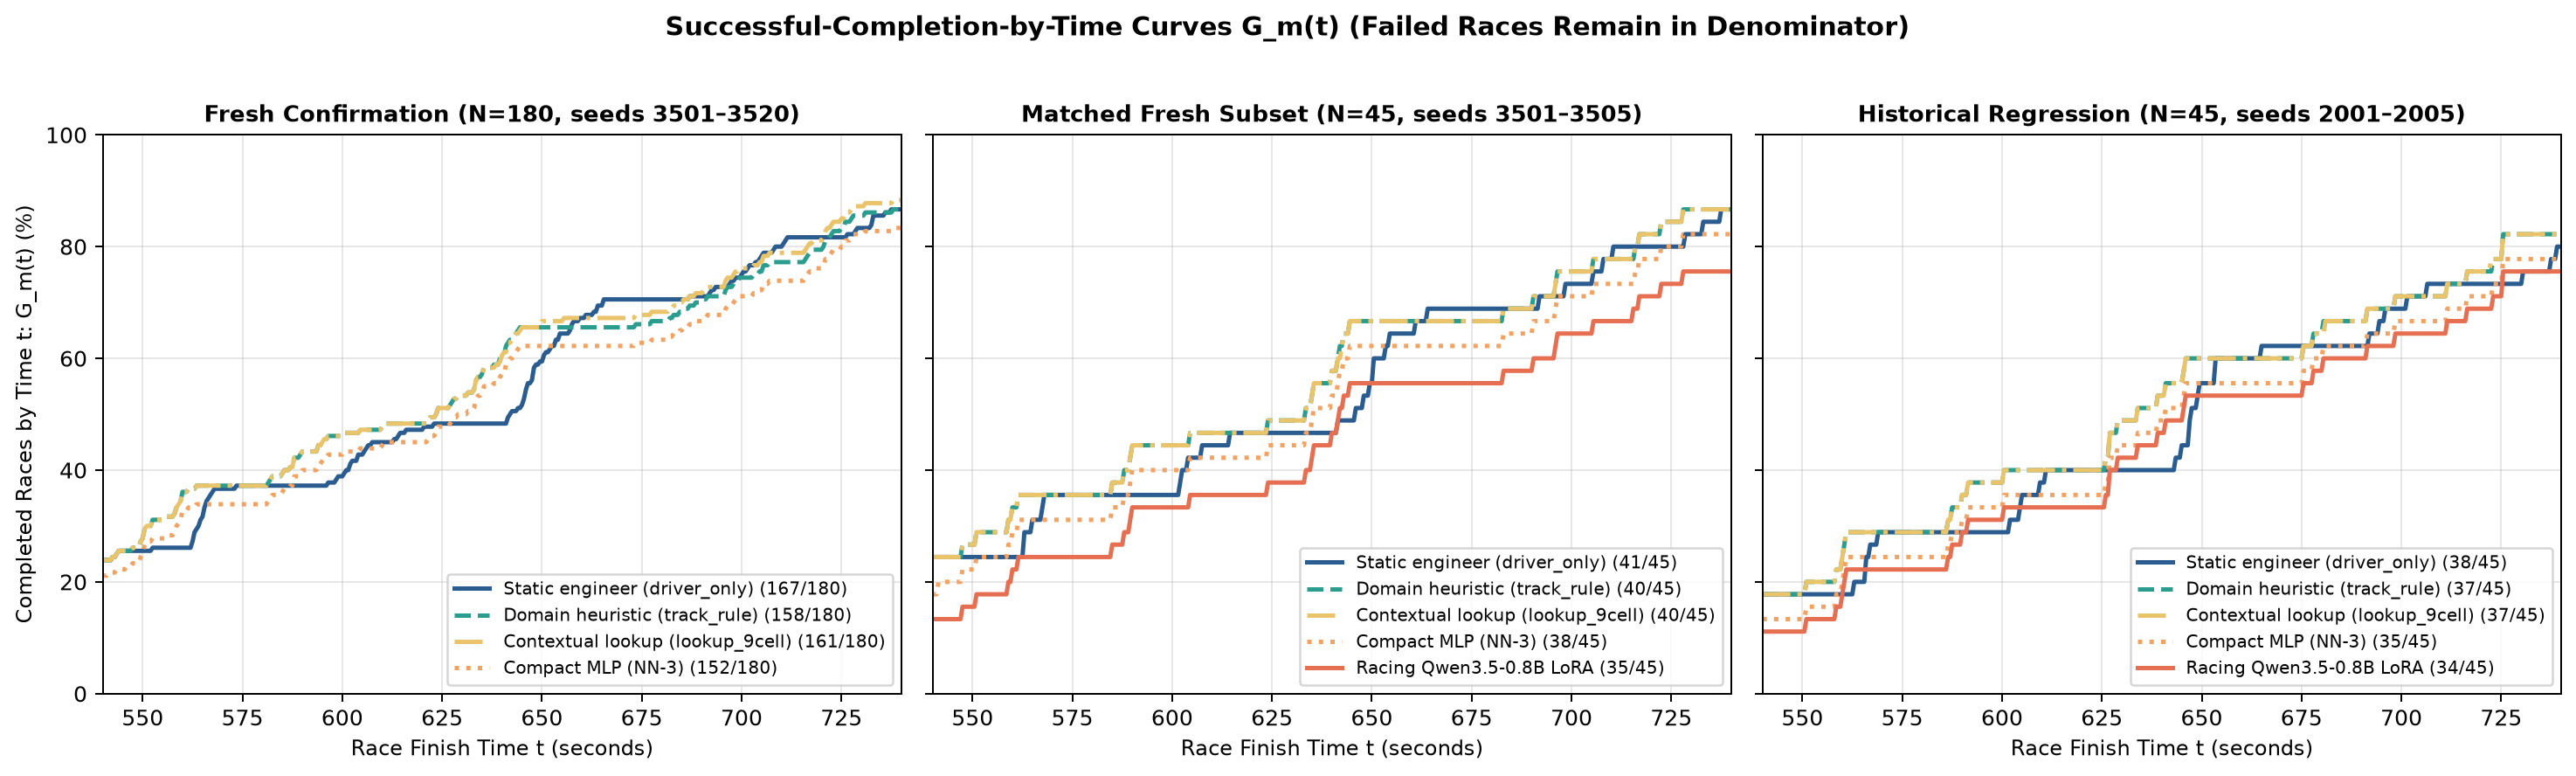
\includegraphics[width=\textwidth]{figures/completion_by_time_curves.png}
\caption{Successful-completion-by-time curves $\widehat{G}_m(t)$ across Fresh-180, Matched Fresh-45, and Historical-45 panels. Failed races remain in the denominator: the right plateau shows completion rate while horizontal position shows timing. Note: \texttt{Racing Qwen} curves reflect the evaluated $512$-token live-lap pace pipeline, where pace prompts were right-truncated within Option~D and lost the \texttt{Answer:} cue during both training and inference (Section~3.6).}
\label{fig:completion_by_time}
\end{figure}

\subsection{Post-Hoc Stage-B Alignment on \texttt{3501..3505} (\texorpdfstring{$N=45$}{N=45}) and Qwen Input-Validity Audit}

To directly compare the racing-trained policies against frozen Study~1/Study~3 references and the exact raw Qwen base initialization under the identical pit-free Stage-B contract (\texttt{pits\_enabled=False}, \nolinkurl{action_spec_hash=a65f275a8fff3740}), we conducted a \textbf{post-hoc evaluation of frozen models on the previously inspected 45-case confirmation subset} (\texttt{3501..3505}, Table~\ref{tab:study2_align45}; saved separately in \texttt{reports/alignment\_supplement/}). All five alignment models---\texttt{kev-0.8b}, off-the-shelf \nolinkurl{cross-encoder/ms-marco-MiniLM-L6-v2}, exact raw \texttt{Qwen/Qwen3.5-0.8B-Base}, Study~1B's \texttt{m2-qwen3.5-0.8b-lora-s42}, and the dated cloud \texttt{frontier-llm} reference (\texttt{deepseek-v4.1-flash-1017})---were run once with zero tuning and paired against the reused frozen \texttt{3501..3505} logs for \texttt{driver\_only}, \texttt{track\_rule}, \texttt{lookup\_9cell}, \texttt{NN-3}, and \texttt{Racing Qwen}.

\begin{table}[t]
\centering
\caption{Study~2 (Post-Hoc Stage-B Alignment Supplement): Complete 10-model comparison on the previously inspected \texttt{3501..3505} subset ($N=45$, pit-free Stage~B, all-model common finishers $n=30$). Top 5 rows reuse frozen \texttt{racing\_engineer\_v1} logs; bottom 5 rows are post-hoc frozen-model runs under the identical contract. $^{\dagger}$Live-lap pace prompts exceeded $512$ tokens and were right-truncated within Option~D, removing the \texttt{Answer:} cue (affecting \texttt{Racing Qwen} pace training as well as live scoring for all three Qwen pipelines); retained as outcomes of the evaluated pipelines.}
\label{tab:study2_align45}
\resizebox{\textwidth}{!}{%
\begin{tabular}{lccccc}
\toprule
System & Completion & Mean Time & Common & Paired vs.\ Static (\texttt{driver\_only}) & Primary Action Pattern \\
 & & (Finishers) & ($n=30$) & (b/r/reg/bf; $\Delta t$ [95\% CI]) & (Builds / Pace Modes) \\
\midrule
Static engineer (\texttt{driver\_only}) & 41/45 (91.11\%) & 617.06 s & 627.74 s & --- & 45 \texttt{dry\_bal} / 172 \texttt{bal} \\
Domain heuristic (\texttt{track\_rule}) & 40/45 (88.89\%) & 607.33 s & 619.28 s & 40/0/1/4; $-$8.573 s [$-$9.636, $-$7.507] & 45 \texttt{dry\_bal} / 118 \texttt{push}, 52 \texttt{bal} \\
Contextual lookup (\texttt{lookup\_9cell}) & 40/45 (88.89\%) & 607.34 s & 619.30 s & 40/0/1/4; $-$8.562 s [$-$9.619, $-$7.497] & 40 \texttt{dry\_bal}, 5 \texttt{wet} / rule pace \\
Compact MLP (\texttt{nn3\_racing\_v1}) & 38/45 (84.44\%) & 612.07 s & 619.31 s & 38/0/3/4; $-$8.957 s [$-$10.364, $-$7.643] & 45 \texttt{dry\_bal} / 142 \texttt{push}, 17 \texttt{bal}, 9 \texttt{cons} \\
\texttt{Racing Qwen LoRA}$^{\dagger}$ (s2026) & 35/45 (77.78\%) & 621.18 s & 619.09 s & 35/0/6/4; $-$9.952 s [$-$11.341, $-$8.603] & 45 \texttt{dry\_bal} / 154 \texttt{push\_max} (100\%) \\
\midrule
\texttt{frontier-llm} (dated cloud, post-hoc) & 39/45 (86.67\%) & 621.72 s & 630.25 s & 39/0/2/4; +2.522 s [+1.833, +3.168] & 30 \texttt{wet}, 8 \texttt{dry\_low}, 7 \texttt{dry\_bal} / 141 \texttt{bal}, 19 \texttt{cons}, 7 \texttt{wet} \\
\texttt{M2 Ops Qwen LoRA}$^{\dagger}$ (s42, post-hoc) & 38/45 (84.44\%) & 626.06 s & 639.94 s & 38/0/3/4; +12.072 s [+11.740, +12.410] & 45 \texttt{dry\_low} / 155 \texttt{cons}, 11 \texttt{wet}, 6 \texttt{bal} \\
\texttt{Raw Qwen Base}$^{\dagger}$ (post-hoc) & 37/45 (82.22\%) & 630.07 s & 640.52 s & 37/0/4/4; +12.665 s [+12.218, +13.148] & 45 \texttt{dry\_low} / 150 \texttt{cons}, 21 \texttt{wet}, 1 \texttt{push} \\
Off-the-shelf MiniLM (post-hoc) & 37/45 (82.22\%) & 629.77 s & 633.31 s & 37/0/4/4; +5.126 s [+4.375, +5.824] & 31 \texttt{damp}, 14 \texttt{dry\_bal} / 164 \texttt{bal} \\
\texttt{kev-0.8b} (post-hoc) & 37/45 (82.22\%) & 624.99 s & 645.11 s & 36/1/5/3; +16.018 s [+15.263, +16.713] & 30 \texttt{dry\_bal}, 15 \texttt{dry\_low} / 158 \texttt{wet}, 16 \texttt{bal} \\
\bottomrule
\end{tabular}}
\end{table}

\paragraph{Dated Cloud Reference Provenance.}
\texttt{frontier-llm} was evaluated on \texttt{2026-11-26} UTC via the configured OpenAI-compatible MaaS endpoint (requested and returned model \texttt{deepseek-v4.1-flash-1017} on all $213/213$ calls; \texttt{temperature=0.0}, \texttt{max\_tokens=128}, \nolinkurl{response_format=json_object}, \nolinkurl{enable_thinking=false}; $0$ invalid outputs, $0$ retries, $0$ truncated calls; $115{,}089$ prompt / $3{,}408$ completion tokens; p50 $639.71$\,ms, p95 $945.69$\,ms, wall $278.8$\,s; full logs in \nolinkurl{reports/alignment_supplement/frontier_stage_b_45_calls.jsonl}). Because hosted services can undergo unannounced serving changes whose magnitude is not established, this row represents a dated cloud reference rather than a guaranteed immutable replica of earlier runs. Notably, even this cloud reference ($39/45$, $0$ rescues / $2$ regressions vs.\ \texttt{driver\_only}, $+2.522$\,s; $0$ rescues / $1$ regression vs.\ \texttt{track\_rule}, $+11.314$\,s) finished more races than every local AI model, yet none of the AI models achieved a higher observed completion count than \texttt{driver\_only} ($41/45$), \texttt{track\_rule} ($40/45$), or \texttt{lookup\_9cell} ($40/45$) on this matched panel.

\paragraph{Qwen Pipeline Contrasts and Input-Validity Audit.}
Comparing the three Qwen pipelines under the identical observation renderer, letter-logit interface (\texttt{letter\_ids = [357, 417, 351, 414, 458]}), and \texttt{max\_length = 512} budget \textbf{compares the frozen checkpoints under the same configured input and scoring pipeline}:
\begin{itemize}[leftmargin=1.5em,itemsep=2pt]
  \item \textbf{\texttt{Racing Qwen} vs.\ \texttt{Raw Qwen Base}:} $-4.44$\,pp completion ($35/45$ vs.\ $37/45$; 95\% CI $[-11.11, +2.22]$; $32$ both finish, $3$ rescues, $5$ regressions, $5$ both fail) and $-21.862$\,s conditional timing ($n=32$, $[-23.074, -20.586]$). Under the evaluated interface, Racing LoRA shifted the action pattern from the raw base's conservative \texttt{dry\_low\_drag} + \texttt{conserve\_tyres} selections ($3$ timeouts, $5$ crashes, $+12.7$\,s slower than static) to $100\%$ \texttt{dry\_balanced} + \texttt{push\_max} ($10$ wall crashes, $-9.95$\,s faster on survivors).
  \item \textbf{\texttt{M2 Ops Qwen LoRA} vs.\ \texttt{Raw Qwen Base}:} $+2.22$\,pp completion ($38/45$ vs.\ $37/45$; $[0.00, +6.67]$; $1$ rescue, $0$ regressions, exact McNemar $p = 1.00$) and $-0.496$\,s ($n=37$, $[-0.848, -0.191]$), retaining nearly the same conservative build/pace pattern as the base.
  \item \textbf{\texttt{Racing Qwen} vs.\ \texttt{M2 Ops Qwen LoRA}:} $-6.67$\,pp completion ($35/45$ vs.\ $38/45$; $[-15.56, 0.00]$; $3$ rescues, $6$ regressions) and $-21.324$\,s ($n=32$, $[-22.609, -19.953]$).
\end{itemize}

\paragraph{Input-Validity Audit of the 512-Token Cap.}
Full BPE tokenization using the saved \texttt{Qwen/Qwen3.5-0.8B-Base} \texttt{tokenizer.json} pipeline (revision \texttt{dc7cdfe2ee4154fa}, \texttt{NFC} normalizer, Split+ByteLevel pre-tokenizer, full BPE vocabulary/merges, ByteLevel post-processor with \texttt{bos\_token=None} adding $0$ special tokens, \texttt{truncation=True}, \texttt{truncation\_side="right"}, \texttt{max\_length=512}) on the rendered Stage-B prompts (matching both \texttt{M2QwenLoRARunner} and \texttt{train\_racing\_v1\_students.py}) reveals a critical distinction between build and pace calls:
\begin{itemize}[leftmargin=1.5em,itemsep=2pt]
  \item \textbf{Pre-race build calls ($0/45$ truncated across all three Qwen models):} Untruncated prompt lengths are $493$--$495$ tokens ($<512$). All forecast fields, the question, all four options (\texttt{A}--\texttt{D}) with full descriptions, and the closing \texttt{Answer:} cue survived intact; with batch size~$1$ (no padding), \nolinkurl{logits[0, -1, letter_ids]} read the intended next-token position immediately after \texttt{Answer:}.
  \item \textbf{Live-lap pace calls ($100\%$ of pace prompts exceeded $512$ tokens, with $22$--$28$ tokens discarded per prompt):} Untruncated pace prompt lengths are $534$--$540$ model tokens, so every live-lap pace call strictly exceeded the $512$-token cap (none merely equaled $512$ without removal): \textbf{$172/172$} pace calls for \texttt{Raw Qwen Base}, \textbf{$172/172$} for \texttt{M2 Ops Qwen LoRA}, and \textbf{$154/154$} on Matched Fresh-45 (\textbf{$150/150$} on Historical-45) for \texttt{Racing Qwen LoRA}, while \texttt{Racing Qwen} training used the same \texttt{max\_length=512} truncation path (\texttt{train\_racing\_v1\_students.py}). By contrast, \texttt{kev-0.8b}, off-the-shelf MiniLM, and \texttt{frontier-llm} had $0$ truncated calls.
  \item \textbf{What survived vs.\ what was removed (scoring-interface defect):} Because right-truncation removed the prompt suffix, \textbf{zero telemetry fields were removed} and the \texttt{Question:} line plus Options~\texttt{A}, \texttt{B}, and~\texttt{C} survived intact. However, right-truncation clipped Option~\texttt{D} (\texttt{wet\_caution}) mid-description and \textbf{removed the entire closing instruction (``\emph{Select the single best option letter (A--D).}'') and \texttt{Answer:} cue}. Although batch size~$1$ ensured no padding tokens were present, \nolinkurl{logits[0, -1, letter_ids]} read the last non-padding token \emph{mid-description inside Option~D} rather than at the intended \texttt{Answer:} boundary. The evaluation-time audit used the fixed candidate order, in which \texttt{wet\_caution} occupied position~\texttt{D}; racing training applied the same $512$-token cap with permuted candidate order, so the semantic action occupying position~\texttt{D} varied across augmented training examples (and this audit verified the shared truncation path rather than every augmented training input individually). Consequently, while pre-race build decisions remain a valid comparison, the live-lap pace results across all three Qwen models reflect a \textbf{scoring-interface truncation defect} in the configured $512$-token pipeline and should not be interpreted as a clean test of Qwen's untruncated live-lap decision-making capability.
\end{itemize}

\subsection{Live Policy Behavior and Causal Restraint}

Three empirical findings stand out from Study~2:
\begin{enumerate}[leftmargin=1.5em,itemsep=2pt]
  \item \textbf{Constant-action execution by \texttt{Racing Qwen}:} Across every live race ($45/45$ builds and $150/150$ laps on Historical-45; $45/45$ builds and $154/154$ laps on Matched Fresh-45), \texttt{Racing Qwen} selected \texttt{dry\_balanced} and \texttt{push\_max} on $100\%$ of calls (while \texttt{stay\_out} was enforced by the pit-free Stage-B contract). On Matched Fresh-45, this yielded $5$ regressions ($0$ rescues) vs.\ \texttt{track\_rule}, $6$ regressions vs.\ \texttt{driver\_only}, and $2$ fewer finishes than its own raw base ($35/45$ vs.\ $37/45$), with no established timing edge over \texttt{track\_rule} ($-0.154$\,s, 95\% CI $[-0.680, +0.262]$; seed-block 95\% CI $[-0.715, +0.290]$).
  \item \textbf{Tiny conditional speed gains versus material completion losses for \texttt{NN-3}:} On Fresh-180, \texttt{NN-3} retained partial pace modulation ($573$ \texttt{push\_max}, $79$ \texttt{balanced}, $29$ \texttt{conserve\_tyres}), achieving a $-0.278$\,s conditional difference vs.\ \texttt{track\_rule} ($\approx 0.046\%$ of a $603$\,s race; 95\% CI $[-0.518, -0.049]$; failure-aware W--T--L at $0.5$\,s tolerance: $13$\,W / $128$\,$T_{\text{fin}}$ / $22$\,$T_{\text{bf}}$ / $17$\,L) at the cost of $6$ fewer finishes vs.\ \texttt{track\_rule} and $15$ fewer finishes vs.\ \texttt{driver\_only}.
  \item \textbf{Observed completion improvement for contextual lookup:} On Fresh-180, \texttt{lookup\_9cell} achieved $3$ rescues and $0$ regressions vs.\ \texttt{track\_rule} ($161/180$ vs.\ $158/180$, $+1.67$\,pp, 95\% CI $[0.00, +3.33]$; descriptive exact two-sided McNemar $p = 0.25$) with virtually identical timing ($+0.012$\,s, $[-0.001, +0.027]$). Three discordant races remain modest evidence rather than an established population-level advantage.
\end{enumerate}

Strong acceptable-set concentration of \texttt{push\_max} ($85.67\%$ of eligible \texttt{train} pace rows), the live-lap right-truncation defect at $512$ tokens (for Qwen), and sequential state-distribution shift~\cite{ross2011dagger} (where earlier \texttt{push\_max} laps move the car off \texttt{track\_rule}'s \texttt{parkland} trajectory) are \textbf{plausible contributors} to the observed constant-action collapse and completion loss, though the present experiments do not isolate their individual causal weights.

% ============================================================================
\section{Study 3: In-Context Feedback and Closed-Loop Reliability}
% ============================================================================

Study~3 addresses a complementary question: how does prior-race context affect closed-loop outcomes when model weights remain fixed? Its \texttt{F1 v2} cohort was defined before the M2 and dedicated racing-training studies; the phased execution of its comparison arms is described below.

As executed, the cohort comprised three scoring interfaces: \texttt{frontier-llm} (\texttt{deepseek-v4.1-flash-1017}) as a cloud generative reference, \texttt{kev-0.8b} as a local pointer-based decision scorer, and off-the-shelf \nolinkurl{cross-encoder/ms-marco-MiniLM-L6-v2} (loaded under the display label \texttt{self-jev-minilm}) as a lightweight ($22.7$M) cross-encoder. Under the original pits-enabled \texttt{RaceEnv} contract, the study compared no history ($Z$), actions-only history ($A$), and factual outcome-feedback history ($F$) on matched \texttt{seed\_B} races (\texttt{2001..2005}, $N=45$), using prior-race context from \texttt{seed\_A} (\texttt{1001..1005}).

\paragraph{Internal Chronology and Cohort Scope.}
Within Study~3 itself, arms $A$ and $F$ for \texttt{self-jev-minilm} and \texttt{frontier-llm} were evaluated first (Pass~1), the matched zero-history arm ($Z$) was added as a post-execution diagnostic to separate baseline behavior from history-induced shifts, and \texttt{kev-0.8b} was added as a delayed planned backfill across all three arms. Because this cohort was defined chronologically prior to \texttt{M2 V5} and \texttt{racing\_engineer\_v1}, Study~3 does not establish how the later task-adapted Qwen LoRA checkpoints would respond to in-context feedback (prior task fine-tuning is compatible with frozen-weight in-context evaluation, but was outside this cohort's scope).

\begin{table}[t]
\centering
\caption{Study~3: In-context adaptation without weight updates on \texttt{seed\_B} (\texttt{2001..2005}, $N=45$). \texttt{self-jev-minilm} is the UI display label for off-the-shelf \nolinkurl{cross-encoder/ms-marco-MiniLM-L6-v2} (not fine-tuned for this project).}
\label{tab:study3_f1v2}
\resizebox{\textwidth}{!}{%
\begin{tabular}{lccccc}
\toprule
Fixed-Weight System & $Z$ (No Hist.) & $A$ (Actions Only) & $F$ (Outcome Feedback) & $F$ vs.\ $A$ (resc/reg; $\Delta t$) & $F$ vs.\ $Z$ (resc/reg; $\Delta t$) \\
\midrule
\texttt{kev-0.8b} & 36/45 (631.37 s) & 36/45 (633.78 s) & 36/45 (633.78 s) & 0/0; 0.00 s ($n=36$) & 0/0; +2.40 s ($n=36$) \\
\texttt{self-jev-minilm} & 40/45 (616.38 s) & 25/45 (633.87 s) & 37/45 (637.93 s) & +14/$-$2; $-$43.81 s ($n=23$) & 0/$-$3; +15.68 s ($n=37$) \\
\texttt{frontier-llm} & 30/45 (637.46 s) & 31/45 (639.00 s) & 33/45 (631.67 s) & +2/0; $-$0.12 s ($n=31$) & +3/0; +0.57 s ($n=30$) \\
\bottomrule
\end{tabular}}
\end{table}

Table~\ref{tab:study3_f1v2} shows that observed in-context history effects depended strongly on both the evaluated checkpoint and the information supplied:
\begin{itemize}[leftmargin=1.5em,itemsep=2pt]
  \item For the evaluated \texttt{frontier-llm} checkpoint (\texttt{deepseek-v4.1-flash-1017}) on this 45-case panel, outcome feedback yielded three additional completions over $Z$ ($30 \rightarrow 33/45$; $+3$ rescues, $0$ regressions, exact two-sided McNemar $p = 0.25$) and two over $A$ ($31 \rightarrow 33/45$; $+2$ rescues, $0$ regressions, $p = 0.50$). While consistent in direction, these small discordant counts provide limited evidence on a single panel rather than an established general reliability benefit for frontier models.
  \item \texttt{kev-0.8b} was invariant between $A$ and $F$ ($36/45$, $0.00$\,s) while slowing slightly relative to $Z$ ($+2.40$\,s across $n=36$ common finishers).
  \item Off-the-shelf \texttt{self-jev-minilm} degraded sharply under actions-only history ($40 \rightarrow 25/45$, accompanied by $84$ pit stops rather than $0$ in $Z$) before partially recovering under outcome feedback ($25 \rightarrow 37/45$, accompanied by $23$ pit stops), yet \textbf{remaining below zero-history $Z$ ($37/45$ vs.\ $40/45$; $+15.68$\,s on $n=37$ common finishers)}.
\end{itemize}

% ============================================================================
\section{Limitations and Reproducibility}
% ============================================================================

Several methodological boundaries govern how these results should be interpreted and reproduced:
\begin{enumerate}[leftmargin=1.5em,itemsep=2pt]
  \item \textbf{Repeated development exposure in Study~1A:} The $N=244$ benchmark (\texttt{full\_benchmark\_v2}) was filtered from an earlier 313-item suite inspected across multiple development iterations; its results are exploratory and should not be weighted like the originally held-out \texttt{holdout\_600} split.
  \item \textbf{Post-hoc supplements and phased chronology:} The 10-model Stage-B alignment on \texttt{3501..3505} was run post-hoc on a previously inspected confirmation subset; the off-the-shelf MiniLM row on \texttt{holdout\_600} was evaluated after the original M2 results were known; and Study~3 (\texttt{F1 v2}) combined Pass-1 $A/F$ runs with a post-execution $Z$ diagnostic and a delayed \texttt{kev-0.8b} backfill.
  \item \textbf{Fixed domain and small matched closed-loop panels:} Study~2 and Study~3 evaluate nine fixed $(\text{track}, \text{weather\_regime})$ cells under deterministic physics (\texttt{domain\_rand=False}). Fresh seeds test new environmental realizations of those nine known cells rather than unseen tracks or weather families, and the matched 45-case panels have limited statistical power for small completion differences (e.g., $3/0$ rescues yields exact McNemar $p = 0.25$).
  \item \textbf{Qwen live-lap truncation confound:} Right-truncation at \texttt{max\_length=512} clipped Option~\texttt{D} and removed the \texttt{Answer:} cue on $100\%$ of live-lap Qwen pace calls ($172/172$ for Raw Qwen and M2 Ops Qwen; $154/154$ Fresh-45 and $150/150$ Hist-45 for Racing Qwen in fixed candidate order, with the same $512$-token cap applied under permuted candidate order during Racing Qwen training), whereas pre-race build calls ($493$--$495$ tokens) were intact. Live-lap Qwen results therefore reflect the configured $512$-token pipeline rather than untruncated model capability.
  \item \textbf{Three seeds and calibration-influenced deployment selection:} Both Study~1B and Study~2 trained three seeds per student and selected the single deployment checkpoint by lowest calibrated \texttt{dev} NLL after fitting scalar temperatures on \texttt{cal}. While holdout/confirmation splits remained untouched during selection, fitted temperatures can influence which seed is promoted.
  \item \textbf{Hosted-model version uncertainty:} Cloud calls targeted \texttt{deepseek-v4.1-flash-1017} with \texttt{temperature=0.0} and logged returned model identifiers and token counts, but hosted endpoints can undergo unannounced serving changes across dates.
  \item \textbf{Simulator evidence versus production software reliability:} \texttt{RaceEnv} is a calibrated deterministic bicycle-model testbed (distinct from the companion 4-wheel \texttt{mac\_racing\_sim} reference engine). Demonstrating failure modes in a simulator establishes concrete evaluation risks, but neither simulator success nor simulator failure directly quantifies reliability in production software environments.
\end{enumerate}

% ============================================================================
\section{Cross-Study Synthesis and Conclusion}
% ============================================================================

Across all three studies, our empirical evidence shows why evaluating decision-oriented AI solely on offline decision accuracy is insufficient for reliable software integration:
\begin{itemize}[leftmargin=1.5em,itemsep=2pt]
  \item \textbf{Level~1 (Static Action Selection):} Evaluated local systems trail the frontier reference sharply on the exploratory v2 benchmark ($62.30\%$ vs.\ $95.08\%$), though well-ranked local scorers enable effective cloud cascades ($89.3\%$ at $50.0\%$ actual escalation, whereas under the implemented strict-threshold routing rule ($\text{conf} < \tau$), tied verbalized confidences in \texttt{qwen-0.8b-json} kept actual escalation at $35.66\%$ across requested targets of $40\%$--$90\%$). On the frozen \texttt{holdout\_600} split, task-adapted LoRA closes much of the gap ($91.00\%$, $\text{ECE}=0.030$, $89.8\%$ abstention recall), whereas the tested full fine-tuning configuration of \texttt{BGE-reranker-base} fails to establish a reliable improvement over initialization ($20.72\% \pm 1.02\%$ three-seed mean; selected seed~1024 vs.\ zero-shot $p = 0.3161$).
  \item \textbf{Level~2 (Sequential Intervention):} High offline acceptable-set accuracy ($88.56\%$--$92.79\%$) can coexist with constant-action execution and lower closed-loop completion than simple static or contextual-lookup controls; on the matched 45-case panel, none of the evaluated AI models achieved a higher observed completion count than \texttt{driver\_only} ($41/45$) or \texttt{track\_rule} ($40/45$), even when some learned policies achieved faster conditional times among survivors. For the Qwen racing pipelines specifically, these outcomes include the confirmed $512$-token live-lap pace training/inference truncation defect, so correctly interfaced Qwen racing performance remains unmeasured.
  \item \textbf{Level~3 (In-Context Experience Use):} Without weight updates, outcome-grounded history yielded three additional completions ($30 \rightarrow 33/45$, $p=0.25$) for the evaluated frontier checkpoint on the 45-case feedback panel, whereas actions-only history sharply degraded off-the-shelf MiniLM ($40 \rightarrow 25/45$, accompanied by $84$ pit stops), which remained below zero-history $Z$ even after outcome feedback ($37/45$).
\end{itemize}

Together, these findings establish an empirical boundary under the tested systems and interfaces: strong offline scores and faster successful trajectories did not consistently translate into higher closed-loop completion, making paired static controls, input-validity audits, and separate reporting of completion and conditional timing essential when evaluating discrete AI decision components.

% ============================================================================
\appendix
\section{Prespecified Engineering Promotion Criteria}
% ============================================================================

Preserved verbatim from \texttt{configs/racing\_engineer\_v1.yaml} and separated from the main academic tables above. Reference policies (\texttt{driver\_only}, \texttt{track\_rule}) are not gated.

\begin{table}[htbp]
\centering
\caption{Frozen record of prespecified engineering promotion criteria for \texttt{racing\_engineer\_v1}. Historical-45 required all 6 checks (\texttt{finishes >= 38}, \texttt{reg\_vs\_drv <= 1}, \texttt{dt\_drv <= -5s}, \texttt{dt\_trk <= 0s}, \texttt{illegal == 0}, \texttt{pits == 0}); Fresh Confirmation required all 8 checks (non-negative completion diffs with 95\% lower bound $>-5$\,pp vs.\ both references, plus timing bounds).}
\label{tab:appendix_gates}
\footnotesize
\begin{tabular}{ll>{\raggedright\arraybackslash}p{4.0cm}>{\raggedright\arraybackslash}p{6.0cm}}
\toprule
Panel & Candidate & Promotion Outcome & Specific Criteria Missed \\
\midrule
Historical-45 & \texttt{lookup\_9cell} & Did not meet prespecified criteria & \texttt{finishes\_ge\_38} (37/45), \texttt{mean\_delta\_vs\_track\_rule\_le\_0s} (+0.018 s) \\
Historical-45 & \texttt{nn3\_racing\_v1} & Did not meet prespecified criteria & \texttt{finishes\_ge\_38} (35/45), \texttt{regressions\_vs\_driver\_le\_1} (3) \\
Historical-45 & \texttt{qwen\_lora\_racing\_v1} & Did not meet prespecified criteria & \texttt{finishes\_ge\_38} (34/45), \texttt{regressions\_vs\_driver\_le\_1} (4) \\
\midrule
Fresh Confirm (180) & \texttt{lookup\_9cell} & Did not meet prespecified criteria & \texttt{comp\_diff\_vs\_driver\_ge\_0} ($-$3.33 pp), \texttt{time\_delta\_vs\_track\_rule\_le\_0s} (+0.012 s) \\
Fresh Confirm (180) & \texttt{nn3\_racing\_v1} & Did not meet prespecified criteria & All four completion criteria ($-$8.33 pp vs.\ \texttt{driver\_only}; $-$3.33 pp vs.\ \texttt{track\_rule}) \\
Fresh Confirm (45) & \texttt{qwen\_lora\_racing\_v1} & Did not meet prespecified criteria & All four completion criteria ($-$13.33 pp vs.\ \texttt{driver\_only}; $-$11.11 pp vs.\ \texttt{track\_rule}) \\
\bottomrule
\end{tabular}
\end{table}

% ============================================================================
\begin{thebibliography}{9}

\bibitem{ross2011dagger}
S.~Ross, G.~J. Gordon, and D.~Bagnell,
``A Reduction of Imitation Learning and Structured Prediction to No-Regret Online Learning,''
in \emph{Proceedings of the 14th International Conference on Artificial Intelligence and Statistics (AISTATS)}, PMLR 15:627--635, 2011.

\bibitem{guo2017calibration}
C.~Guo, G.~Pleiss, Y.~Sun, and K.~Q. Weinberger,
``On Calibration of Modern Neural Networks,''
in \emph{Proceedings of the 34th International Conference on Machine Learning (ICML)}, PMLR 70:1321--1330, 2017.

\bibitem{geifman2017selective}
Y.~Geifman and R.~El-Yaniv,
``Selective Classification for Deep Neural Networks,''
in \emph{Advances in Neural Information Processing Systems (NeurIPS)}, vol.~30, 2017.

\bibitem{hu2022lora}
E.~J. Hu, Y.~Shen, P.~Wallis, Z.~Allen-Zhu, Y.~Li, S.~Wang, L.~Wang, and W.~Chen,
``LoRA: Low-Rank Adaptation of Large Language Models,''
in \emph{International Conference on Learning Representations (ICLR)}, 2022, arXiv:2106.09685.

\bibitem{minilm_card}
Sentence-Transformers / Hugging Face Model Card,
``\texttt{cross-encoder/ms-marco-MiniLM-L6-v2},''
\url{https://huggingface.co/cross-encoder/ms-marco-MiniLM-L6-v2}.

\end{thebibliography}

\end{document}
